% figure: 现控1-9-模拟结构图.png
% Controllable companion realization with three integrators.
\documentclass[border=10pt]{standalone}
\usepackage{fontspec}
\setmainfont{Cambria}
\usepackage{unicode-math}
\setmathfont{Cambria Math}
\usepackage{tikz}
\usetikzlibrary{arrows.meta}
\begin{document}
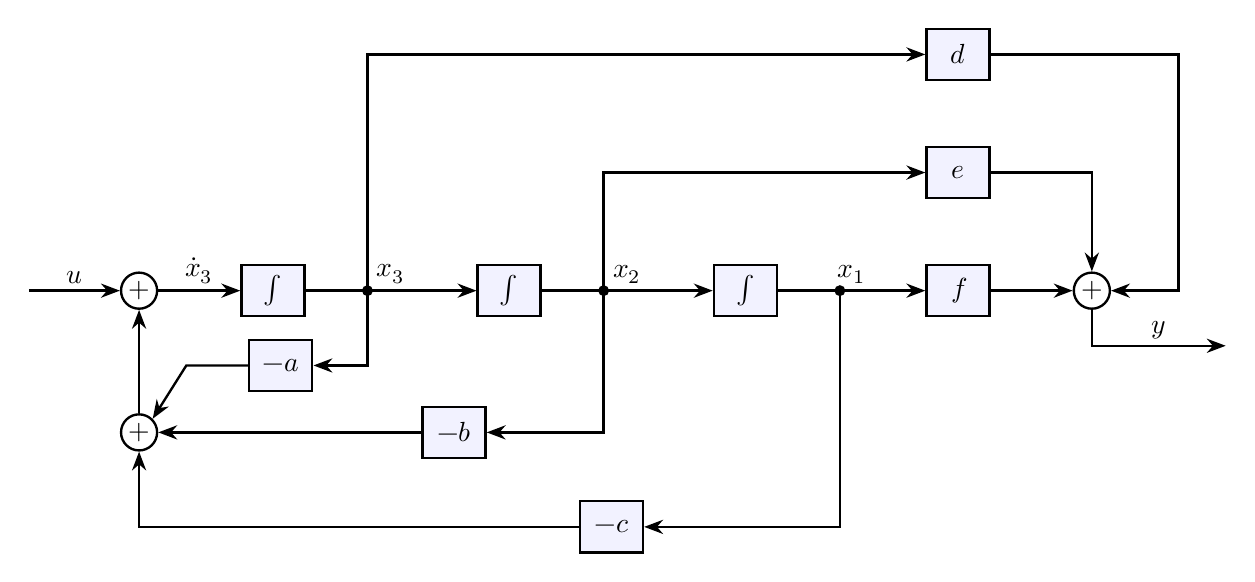
\begin{tikzpicture}[>=Stealth,line width=0.85pt,
 b/.style={draw,minimum width=0.8cm,minimum height=0.65cm,fill=blue!5},
 sum/.style={draw,circle,inner sep=1pt,minimum size=0.4cm},
 lab/.style={fill=white,inner sep=2pt},dot/.style={circle,fill,inner sep=1.4pt}]
\node[sum] (s) at (0,0) {$+$};
\node[b] (i3) at (1.7,0) {$\int$};
\node[b] (i2) at (4.7,0) {$\int$};
\node[b] (i1) at (7.7,0) {$\int$};
\node[b] (gf) at (10.4,0) {$f$};
\node[sum] (o) at (12.1,0) {$+$};
\node[sum] (fb) at (0,-1.8) {$+$};
\node[b] (ma) at (1.8,-0.95) {$-a$};
\node[b] (mb) at (4,-1.8) {$-b$};
\node[b] (mc) at (6,-3) {$-c$};
\node[b] (ge) at (10.4,1.5) {$e$};
\node[b] (gd) at (10.4,3) {$d$};
\draw[->] (-1.4,0) -- node[lab,above] {$u$} (s);
\draw[->] (s) -- node[lab,above] {$\dot x_3$} (i3);
\draw[->] (i3) -- node[lab,above] {$x_3$} (i2);
\draw[->] (i2) -- node[lab,above] {$x_2$} (i1);
\draw[->] (i1) -- node[lab,above] {$x_1$} (gf);
\draw[->] (gf) -- (o);
\draw[->] (o.south) -- (12.1,-0.7) -- node[lab,above] {$y$} (13.8,-0.7);
\node[dot] at (2.9,0) {};
\node[dot] at (5.9,0) {};
\node[dot] at (8.9,0) {};
\draw[->] (2.9,0) -- (2.9,-0.95) -- (ma.east);
\draw[->] (ma.west) -- (0.6,-0.95) -- (fb.north east);
\draw[->] (5.9,0) -- (5.9,-1.8) -- (mb.east);
\draw[->] (mb.west) -- (fb.east);
\draw[->] (8.9,0) -- (8.9,-3) -- (mc.east);
\draw[->] (mc.west) -- (0,-3) -- (fb.south);
\draw[->] (fb.north) -- (s.south);
\draw[->] (5.9,0) -- (5.9,1.5) -- (ge.west);
\draw[->] (ge.east) -- (12.1,1.5) -- (o.north);
\draw[->] (2.9,0) -- (2.9,3) -- (gd.west);
\draw[->] (gd.east) -- (13.2,3) -- (13.2,0) -- (o.east);
\end{tikzpicture}
\end{document}
